%%%%%%%%%%%%%%%%%%%%%%%%%%%%%%%%%%%%%%%%%%%%%%%%%%%%%%%%%%%%%%%%%%%%%%%%%%%
%
% Plantilla para un artículo en LaTeX en español.
%
%%%%%%%%%%%%%%%%%%%%%%%%%%%%%%%%%%%%%%%%%%%%%%%%%%%%%%%%%%%%%%%%%%%%%%%%%%%



%--------------------------------------------------------------------------
\title{Plantilla para un artículo \LaTeX}
\author{El autor va aquí\\
  \small Dept. Plantillas y Editores\\
  \small E12345\\
  \small España
}

\begin{document}
\section{Resumen}
\item{Estamos acostumbrados a tablas dinámicas y  ahora, las nuevas herramientas de visualización de datos como Tableau o Qlikview tienen mucha aceptación porque puedes jugar con los datos, ver cómo cambian las previsiones o los resultados según combinas las variables. Todo con colores y muy visual. Vamos, que queda muy chulo ver un cuadro de mandos con colorines y mapas en 3D y todo eso, pero nos encontraremos con un problema gordo y es que, según en un post previo las empresas que están invirtiendo en analítica predictiva (integrar diferentes datos para predecir el mercado) siguen teniendo problemas a la hora de desarrollar acciones para los insights que les están dando los diferentes algoritmos.

Esto no es más que, pese a que tienen datos súper molones, no entienden bien lo que los datos les están contando. Y he aquí la solución: hacer de los datos algo con lo que la persona de negocio sienta relación. Aquí entra, ni más ni menos que el denominado Storytelling con datos  o historias que generen un impacto o un cambio en las acciones de una persona basado en los resultados de un análisis.

En las antiguas civilizaciones, los jefes de los pueblos realizaban preguntas a los oráculos para poder saber qué hacer (invadir un pueblo cercano, responder o no a las amenazas de otros dirigentes…) Luego, los oráculos (no sabemos si puestos hasta arriba de algún alucinógeno) daban respuestas de lo más creativas que dejaba al jefe con los deberes de interpretar lo que el oráculo había dicho.

\section{Abstract}
\item{We are used to dynamic tables and now, the new data visualization tools such as Tableau or Qlikview are very popular because you can play with the data, see how the forecasts or results change as you combine the variables. All with colors and very visual. Come on, it is very cool to see a dashboard with colorines and 3D maps and all that, but we will have a big problem and that is, according to a previous post companies that are investing in predictive analytics (integrate different data to predict the market) continue to have problems when developing actions for the insights that the different algorithms are giving them.

This is just that, although they have super cool data, they do not understand what the data is telling them. And here's the solution: make the data something that the business person feels connected to. Here it enters, neither more nor less than the so-called Storytelling with data or stories that generate an impact or a change in the actions of a person based on the results of an analysis.

In the old civilizations, the heads of the towns asked questions to the oracles to know what to do (invade a nearby town, respond or not to the threats of other leaders ...) Then, the oracles (we do not know if they put up some hallucinogen) gave the most creative answers that left the boss with the duties of interpreting what the oracle had said.
\newpage

\section{Introduccion}
\item{La Narrativa en la Visualización de Datos es una de las principales herramientas del Big Data que los negocios no se pueden perder.Por eso, en este post te contamos lo más interesante del DataStorytelling, qué es y cómo mejorar los resultados gracias a ello.\\\\
Por si no lo sabías, cada vez se van a necesitar más profesionales big data y  storytelleres en el sector. El cambio en la era digital demanda perfiles con capacidades analíticas y de inteligencia empresarial. Como consecuencia, las nuevas generaciones irán más allá de estas disciplinas, con nuevas ideas y espacios para los negocios.}

\section{DATA STORYTELLYNG}
\item{La narración de datos o el DataStorytelling es el proceso de traducir los análisis de datos a términos simples para influir en una decisión o acción comercial. Este término se ha asociado con diferentes funciones: visualizaciones de datos, infografías, tableros, etc. El DataStorytelling es mucho más que eso, son formas de comunicar información con datos, imágenes y narrativa. Con el crecimiento de los negocios digitales, la toma de decisiones basada en los datos se ha convertido en algo primordial a menudo asociado con la analítica y la ciencia de los datos.\\\\
Para comprender mejor qué es el DataStorytelling, hay que centrarse en estos tres elementos (dato, imagen y narrativa) y ver cómo trabajan juntos. Lo que se busca es dar voz a los datos y comunicar los resultados del análisis con narrativas. Es hacer de una presentación aburrida una historia con datos entretenida. Aquello que no llamaba la atención sin elementos visuales como son los  gráficos o las tablas, ahora cobra forma bajo el Storytelling.}
\begin{figure}[htb]
\begin{center}
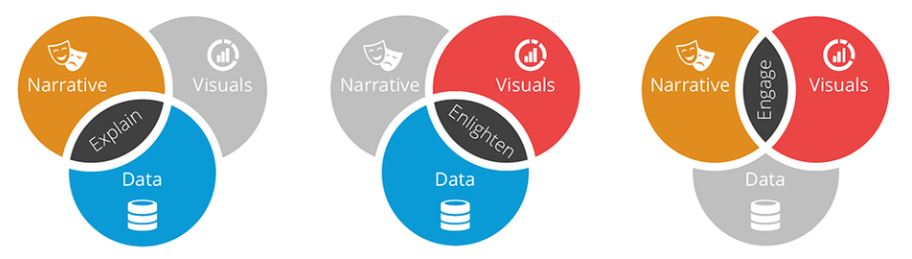
\includegraphics[width=15cm]{./Imagenes/imagen1}
\end{center}
\end{figure}

\item{
Como puedes ver en esta imagen elaborada por Forbes, en cada gráfico las interacciones de los elementos significan cosas diferentes, con resultados particulares. Como resultado vemos las siguientes interacciones:
\\\\1.Narrativa y datos: la combinación de ambos sirve para ofrecer a la audiencia una explicación sobre los mismos.
\\\\2.Visualización y datos: como ves en la imagen, la palabra enlighten (que significa iluminar) es el resultado de la combinación de ambos. Añadir una visualización a los datos ayuda informar de forma entretenida e inteligible.
\\\\3.Narrativa y visualización: esta combinación tiene como resultado la captación de clientes.
\\\\¿Qué ocurre cuando se juntan los tres? Si los elementos están combinados correctamente, el resultado será un datastorytelling que conduzca al cambio positivo del negocio. Lo importante es que la audiencia sea capaz de entender y recordar el mensaje que se quiere transmitir, por eso los profesionales del Big Data y el Storytelling deben conocer bien a sus audiencias para saber qué ofrecer.
}
\section{¿Por qué es necesario el Data Storytelling?}

\item{El profesional en Big Data Philippe Nieuwbourg dice que el objetivo del Data Storytelling es “hacer que las personas se metan en la historia, como en una buena película de cine”. Esto es precisamente lo que busca esta nueva ciencia que combina StoryTelling y Big Data. Varios estudios muestran que el datastorytelling influye positivamente en la memorabilidad, la persuasión y el compromiso. El público, en lugar de analizar los detalles, prefiere ver adónde le lleva la historia y sentirse partícipe de ella.
\\\\“Esto sucede de forma similar en las presentaciones de las organizaciones, por eso cuando vemos en una presentación de diapositivas que pasan unas tras otras, que la gente se aburre (…) el objetivo del Data Storytelling es que la presentación se convierta también tan cautivadora como una película, un libro o inclusive una obra de teatro. Cuando se hacen buenas presentaciones o exposiciones, el héroe de éstas es el espectador, el presentador debe ser capaz de llevar a las personas del auditorio al interior de la historia que presenta”, asegura.
\\\\Las historias siempre han sido herramientas que funcionan muy bien para la experiencia humana. Aquellas que muestran análisis y datos son relativamente versiones de estas experiencias humanas. La narrativa es la forma de simplificar y darle sentido a un mundo complejo, ¿verdad? Aporta al espectador contexto, visión o interpretación. Todas ellas hacen que los datos cobren sentido y la analítica sea más relevante e interesante. Con la analítica, el objetivo de la estrategia es cambiar cómo una persona toma una decisión o pasa a la acción.Lo que se intenta con esto es inspirar confianza y contribuir al cambio con las herramientas del dataStoryTelling. Sin duda, la era digital ha hecho que las historias que incorporan datos y análisis son más convincentes que aquellas basadas sólo en anécdotas o experiencias personales.
}

\section{¿Por qué los datos cuentan el futuro?}

\item{La narración de datos es una metodología para comunicar información, adaptada a una audiencia específica, con una narrativa convincente. Son los últimos diez pies de su análisis de datos y posiblemente el aspecto más importante.

Evolutivamente, como Humanos, naturalmente estamos programados para compartir historias como un medio para compartir información.

Los teóricos incluso sugieren que la narración de historias fue la plataforma de lanzamiento principal para la transmisión de conocimiento entre grandes grupos de personas, que formaron culturas como las conocemos hoy y permitieron el éxito evolutivo a través de generaciones.

Ahora, con tanta información disponible para nosotros, solo la narración de datos puede poner una perspectiva humana en el mundo cada vez más complejo y rápidamente cambiante de la era digital.}

\begin{center}
\caption\textbf{EJEMPLOS BASICOS DE DATA-STORYTELLING}
\end{center}
\\
\begin{itemize}
\item  Corum, un editor de gráficos para el New York Times, tiene un marco descriptivo que contrasta varias consecuencias del storytelling:

		\begin{center}
		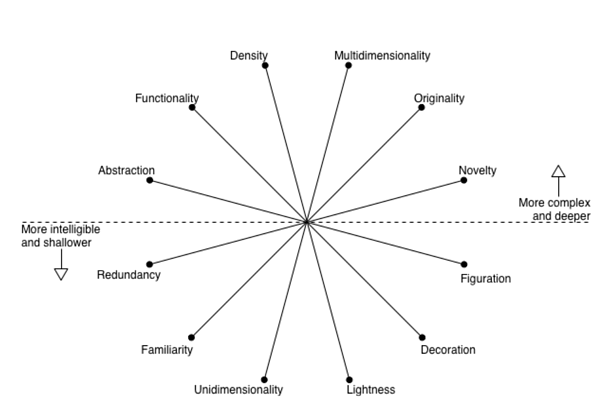
\includegraphics[width=15cm]{./Imagenes/Ejemplo1}
		\end{center}
		
- Densidad vs. ligereza\\
- Multimensionalidad vs. unidimensionalidad\\
- Originalidad vs. familiaridad\\
- Novedad vs. redundancia\\
- Figuración vs. abstracción\\
- Decoración vs. funcionalidad\\

Cada una de estas consecuencias sirve a diferentes propósitos y además se puede presentar usando formatos diferentes.

	\end{itemize}

\section{Ejemplo}

\item{Aquí en Another Company trabajamos con Waze para generar todo tipo de storytelling. Como seguramente sabes, Waze es la aplicación de tráfico y navegación basada en la comunidad más grande del mundo, por lo tanto, su corazón son los datos que sus mismos usuarios generan minuto a minuto mientras navegan en el tráfico de las grandes ciudades. 

La app cuenta con datos de sus usuarios que no solamente dan pie a historias interesantes para la población en general y periodistas, sino que también le han servido para hacer alianzas con los gobiernos para contribuir a la movilidad, a la modernización de las ciudades y al incremento del bienestar de sus consumidores. 

Por ejemplo, hemos generado historias que responden a preguntas como “¿cuál es el comportamiento de los conductores latinoamericanos en el Día de las Madres?” o sobre cómo los datos de los Wazers europeos describen la nueva organización del llamado Viejo Continente. }

\begin{figure}[htb]
\begin{center}
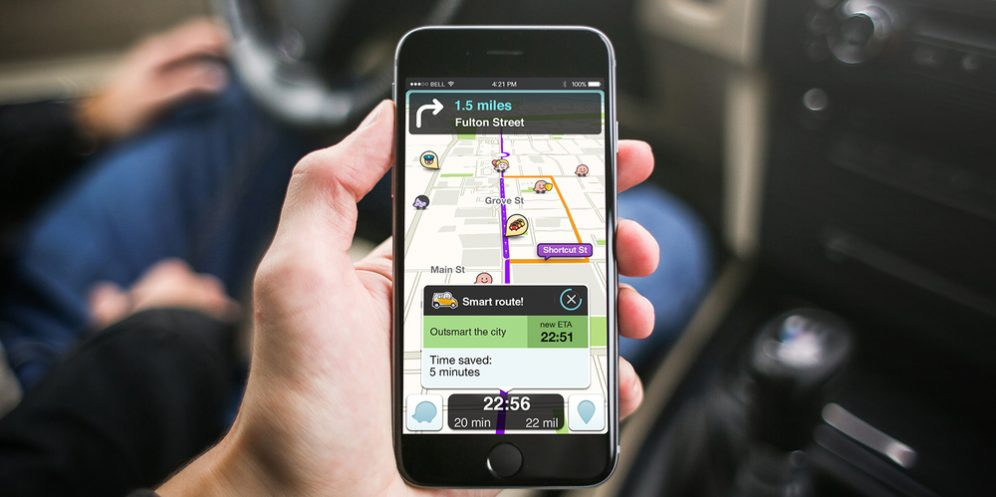
\includegraphics[width=15cm]{./Imagenes/waze2}
\end{center}
\end{figure}

\section{Conclusiones}

\item{Como ves, no necesitas ser un “nerd” obsesionado con los datos para entenderlos y para poner bajo los reflectores el valor de los productos o servicios de tu marca. Para eso estamos nosotros: nuestra tarea es hacer las preguntas correctas, entender los puntos más importantes que aporten significado a los hallazgos y ponerlos en contexto, porque lanzar hechos y cifras aleatorios o liberar tablas de Excel con cientos de filas no funciona. 

Usar la data con efectividad requiere ser selectivo y aterrizar información en el contexto de la narrativa que estás comunicando para amplificar la conversación sobre tu marca que está teniendo lugar en los medios. Todos estos datos tienen que contar una historia, si no no tienen chiste. Acércate a nosotros para aprovechar toda la información con la que cuentas para generar historias de impacto. Tenemos muchas ideas que compartir contigo  }




\newpage
% Bibliografía.
%-----------------------------------------------------------------
\begin{thebibliography}{99}


\bibitem{Cd94} https://www.iebschool.com/blog/data-storytelling-que-es-big-data/
\bibitem{Cd94}  Big Data: A Revolution that Will Transform how We Live, Work, and Think Viktor Mayer-Schonberger y Kenneth Cukier
\bibitem{Cd94}  Storytelling With Data: A Data Visualization Guide for Business Professionals

\end{thebibliography}

\end{document}
